\begin{frame}{FitzHugh-Nagumo model}
	\begin{itemize}
		\item System
		%
		\begin{subequations}
			\begin{align}
				\dot v(t) &= v(t) - \frac{v^3(t)}{3} - w + e, &
				e &= 0.35, \\
				\dot w(t) &= \frac{1}{\tau} v(t) + \frac{a}{\tau} - \frac{b}{\tau} w(t), &
				a    &=  0.7, &
				b    &=  2.0, &
				\tau &= 12.5
			\end{align}
		\end{subequations}
		%
		\item Numerical results (the parameter is $e$, it is increased by 30\%, and the sensitivities have been normalized)
		%
		\vspace{-2pt}
		%
		\begin{center}
			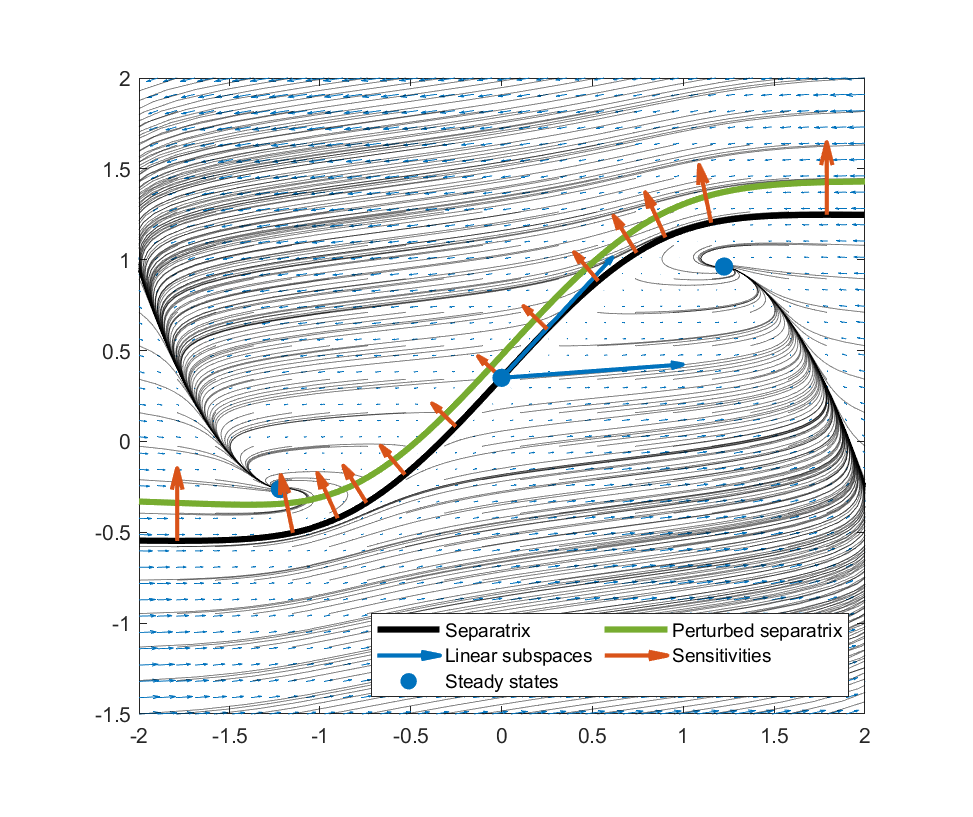
\includegraphics[width=0.7\textwidth, trim=0 0 0 20pt, clip]{./fig/fitzhughnagumo}
		\end{center}
	\end{itemize}
\end{frame}